%!TEX program = xelatex
\documentclass[12pt, a4paper]{article}

\usepackage[dvipsnames]{xcolor}

\usepackage{fancyhdr}
\usepackage{extramarks}
\usepackage{amsmath}
\usepackage{amsthm}
\usepackage{amsfonts}
\usepackage{tikz}
\usepackage[plain]{algorithm}
\usepackage{algpseudocode}

\usepackage{ctex}
\usepackage{indentfirst}
\usepackage{wrapfig}
\usepackage{upgreek}
\usepackage{subfigure}
\ctexset {today=old}
\usetikzlibrary{automata,positioning,shapes.geometric,arrows.meta,patterns,calc}
\numberwithin{equation}{section}

%
% Basic Document Settings
%

\topmargin=-0.25in
\evensidemargin=0in
\oddsidemargin=0in
\textwidth=6.5in
\textheight=9.2in
\headsep=0.25in

\linespread{1.1}

\pagestyle{fancy}
\lhead{\hmwkAuthorName}
\chead{\hmwkClass : \hmwkTitle}
\rhead{\firstxmark}
\lfoot{\lastxmark}
\cfoot{\thepage}

\renewcommand\headrulewidth{0.4pt}
\renewcommand\footrulewidth{0.4pt}

\setlength{\parindent}{2em}  % 2em代表首行缩进两个字符

%
% Create Problem Sections
%

\newcommand{\enterProblemHeader}[1]{
    \nobreak\extramarks{}{Problem \arabic{#1} continued on next page\ldots}\nobreak{}
    \nobreak\extramarks{Problem \arabic{#1} (continued)}{Problem \arabic{#1} continued on next page\ldots}\nobreak{}
}

\newcommand{\exitProblemHeader}[1]{
    \nobreak\extramarks{Problem \arabic{#1} (continued)}{Problem \arabic{#1} continued on next page\ldots}\nobreak{}
    \stepcounter{#1}
    \nobreak\extramarks{Problem \arabic{#1}}{}\nobreak{}
}

% \setcounter{secnumdepth}{0}
\newcounter{partCounter}
\newcounter{homeworkProblemCounter}
\setcounter{homeworkProblemCounter}{0}
% \nobreak\extramarks{Problem \arabic{homeworkProblemCounter}}{}\nobreak{}

%
% Homework Problem Environment
%
% This environment takes an optional argument. When given, it will adjust the
% problem counter. This is useful for when the problems given for your
% assignment aren't sequential. See the last 3 problems of this template for an
% example.
%
\newenvironment{homeworkProblem}[1][-1]{
    \ifnum#1>0
        \setcounter{homeworkProblemCounter}{#1}
    \fi
    \section{Problem \arabic{homeworkProblemCounter}}
    \setcounter{partCounter}{1}
    \enterProblemHeader{homeworkProblemCounter}
}{
    \exitProblemHeader{homeworkProblemCounter}
}

%
% Homework Details
%   - Title
%   - Due date
%   - Class
%   - Section/Time
%   - Instructor
%   - Author
%

\newcommand{\hmwkTitle}{Mechanical Vibration}
\newcommand{\hmwkDueDate}{\today}
\newcommand{\hmwkClass}{University Physics}
\newcommand{\hmwkClassTime}{}
\newcommand{\myUniversiy}{Wuhan University}
\newcommand{\hmwkAuthorName}{\textbf{Lai Wei}}

%
% Title Page
%

\title{
    \vspace{2in}
    \textmd{\textbf{\hmwkClass:\ \hmwkTitle}}\\
    \normalsize\vspace{0.1in}\small{Date: \hmwkDueDate}\\
    \vspace{0.1in}\large{\textit{\myUniversiy}}
    \vspace{3in}
}

\author{\hmwkAuthorName}
\date{}

\renewcommand{\part}[1]{\textbf{\large Part \Alph{partCounter}}\stepcounter{partCounter}\\}

%
% Various Helper Commands
%

% Useful for algorithms
\newcommand{\alg}[1]{\textsc{\bfseries \footnotesize #1}}

% % For derivatives
% \newcommand{\deriv}[1]{\frac{\mathrm{d}}{\mathrm{d}x} (#1)}

% For partial derivatives
\newcommand{\pderiv}[2]{\frac{\partial}{\partial #1} (#2)}

% Integral dx
\newcommand{\dx}{\mathrm{d}x}

% Alias for the Solution section header
\newcommand{\solution}{\textbf{\large Solution}}

% Probability commands: Expectation, Variance, Covariance, Bias
\newcommand{\E}{\mathrm{E}}
\newcommand{\Var}{\mathrm{Var}}
\newcommand{\Cov}{\mathrm{Cov}}
\newcommand{\Bias}{\mathrm{Bias}}

% 我的newcommand
\newcommand{\degree}{^{\circ}}
\newcommand{\arrow}{-{Stealth[length=4mm,width=2mm]}}
\newcommand{\rmd}{\mathrm{~d}}
\newcommand{\deriv}[2]{\frac{\rmd #1}{\rmd #2}}
\renewcommand{\parallel}{\mathrel{/\mskip-2.5mu/}}

\begin{document}

\maketitle

\pagebreak

% 设置页码格式是罗马数字
\pagenumbering{roman}

% 生成目录
\tableofcontents

\newpage 
\mbox{}
\newpage

\pagebreak

% 设置页码格式是阿拉伯数字
\pagenumbering{arabic}

\pagebreak

    机械振动:物体围绕一固定位置往复运动。

\section{简谐振动}

\subsection{简谐振动的动力学特征}

\subsubsection{弹簧振子的振动}

    模型:谐振子轻弹簧(不计质量)与物体(看成质点)

    弹簧振子的无阻尼自由振动:

    \[
        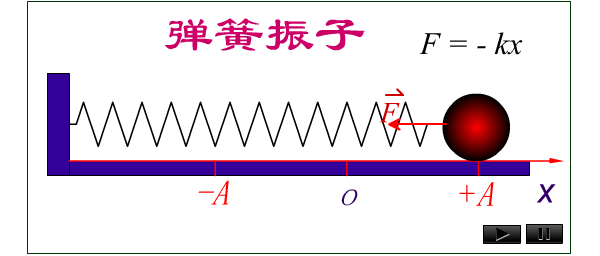
\includegraphics[scale=0.5]{Chapter 06 images/pic1.png}
    \]

    振动的成因:

    \begin{enumerate}
        \item 回复力;
        \item 惯性。
    \end{enumerate}

\subsubsection{弹簧振子的运动方程}

    \begin{equation}
        F=-k x=m a=m \frac{\rmd^2 x}{\rmd t^2}
    \end{equation}

    令
    
    \[
        \omega^2=\frac{k}{m}
    \]
    
    得
    
    \[
        \dfrac{\rmd^2 x}{\rmd t^2} = -\omega^2 x
    \]

    即\(a=-\omega^2 x\)

    具有加速度\(a\)与位移的大小\(x\)成正比,而方向相反特征的振动称为简谐运动。

    简谐运动的微分方程:

    \begin{align}
        \dfrac{\rmd^2 x}{\rmd t^2} = -\omega^2 x
        \label{6-1-2}
    \end{align}

    解得

    \begin{align}
        x = A \cos\left(\omega t + \varphi\right)
    \end{align}

    或

    \begin{align}
        x = A \sin\left(\omega t + \varphi + \frac{\uppi}{2}\right)
    \end{align}

    用复指数表示
    
    \begin{equation}
        x=A \mathrm{e}^{\mathrm{i}(\omega t+\varphi)}
    \end{equation}

    \textbf{公式之间的相互推导关系}

    \[
        \tikzset{every picture/.style={line width=0.75pt}} %set default line width to 0.75pt
        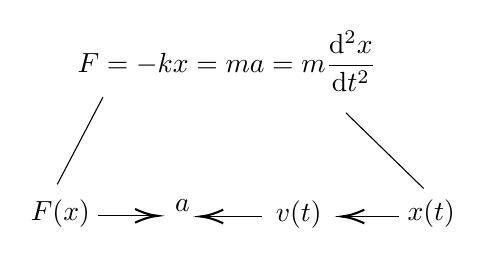
\begin{tikzpicture}[x=0.75pt,y=0.75pt,yscale=-1,xscale=1]
            %uncomment if require: \path (0,300); %set diagram left start at 0, and has height of 300
            %Straight Lines [id:da5445518985427571] 
            \draw    (155.43,153.29) -- (182.43,153.29) ;
            \draw [shift={(184.43,153.29)}, rotate = 180] [color={rgb, 255:red, 0; green, 0; blue, 0 }  ][line width=0.75]
                (10.93,-3.29) .. controls (6.95,-1.4) and (3.31,-0.3) .. (0,0) .. controls (3.31,0.3) and (6.95,1.4) .. (10.93,3.29)   ;
            %Straight Lines [id:da8539578247281134] 
            \draw    (234.5,153.61) -- (207,153.61) ;
            \draw [shift={(205,153.61)}, rotate = 360] [color={rgb, 255:red, 0; green, 0; blue, 0 }  ][line width=0.75]
                (10.93,-3.29) .. controls (6.95,-1.4) and (3.31,-0.3) .. (0,0) .. controls (3.31,0.3) and (6.95,1.4) .. (10.93,3.29)   ;
            %Straight Lines [id:da08053806804260755] 
            \draw    (300.5,153.61) -- (275,153.61) ;
            \draw [shift={(273,153.61)}, rotate = 360] [color={rgb, 255:red, 0; green, 0; blue, 0 }  ][line width=0.75]
                (10.93,-3.29) .. controls (6.95,-1.4) and (3.31,-0.3) .. (0,0) .. controls (3.31,0.3) and (6.95,1.4) .. (10.93,3.29)   ;
            %Straight Lines [id:da2022111052056348] 
            \draw    (158,96.11) -- (136,138.11) ;
            %Straight Lines [id:da9851232959428675] 
            \draw    (275,103.61) -- (312.5,140.11) ;
            % Text Node
            \draw (122,144.4) node [anchor=north west][inner sep=0.75pt]    {$F( x)$};
            \draw (191.5,144.4) node [anchor=north west][inner sep=0.75pt]    {$a$};
            \draw (240,144.9) node [anchor=north west][inner sep=0.75pt]    {$v( t)$};
            \draw (303.5,144.4) node [anchor=north west][inner sep=0.75pt]    {$x( t)$};
            \draw (144.5,62.9) node [anchor=north west][inner sep=0.75pt]    {$F=-kx=ma=m\dfrac{\mathrm{d}^{2} x}{\mathrm{d} t^{2}}$};
        \end{tikzpicture}
    \]

\subsubsection{谐振动的速度和加速度}

    由

    \begin{align*}
        x = A \cos\left(\omega t + \varphi\right)
    \end{align*}

    运动方程对时间求导

    \begin{equation}
        v=\frac{\mathrm{d} x}{\mathrm{~d} t}=-\omega A \sin (\omega t+\varphi)=-v_{\mathrm{m}} \sin (\omega t+\varphi)
    \end{equation}

    运动方程对时间求二阶导

    \begin{equation}
        a=\frac{\mathrm{d}^2 x}{\mathrm{~d} t^2}=-\omega^2 A \cos (\omega t+\varphi)=
        -a_{\mathrm{m}} \cos (\omega t+\varphi)
    \end{equation}

    其中,

    $$
        A=\sqrt{x_0^2+\left(\frac{v_0}{\omega}\right)^2}
    $$

    $$
        \varphi=\arctan \left(-\frac{v_0}{\omega x_0}\right)
    $$

    (此结果一般有两个值,最后要舍去一个,根据速度的方向。)
    
    \[
        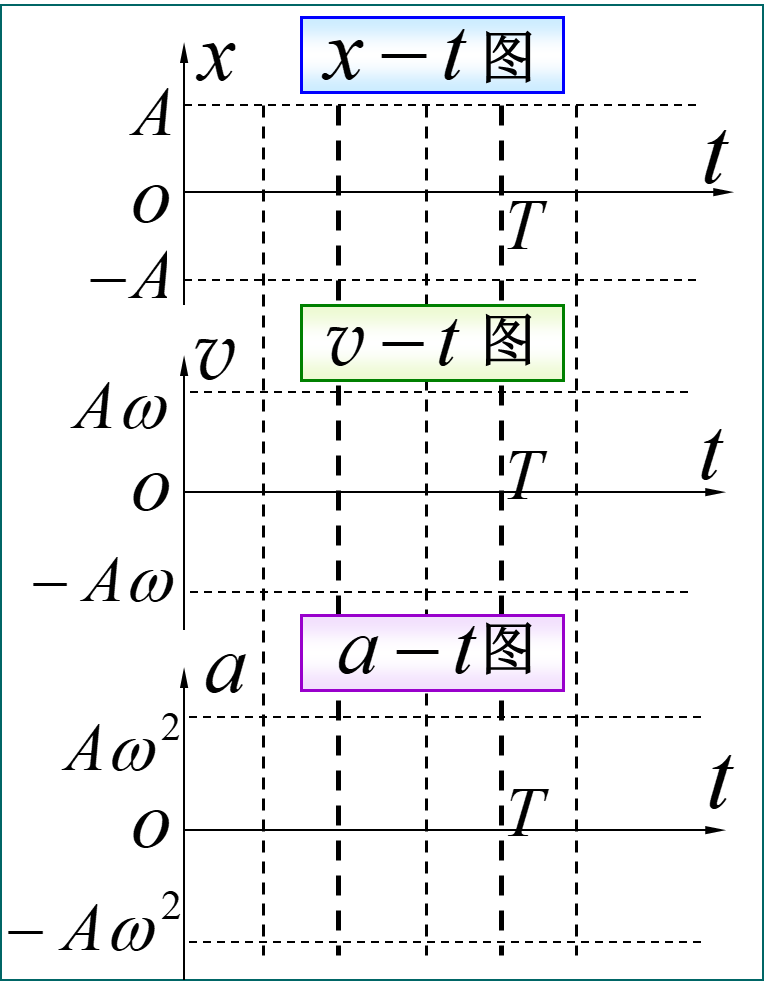
\includegraphics[scale=0.5]{Chapter 06 images/pic2.png}
    \]

\subsubsection{描述简谐振动的物理量}

    振幅 (amplitude):

    \begin{align}
        x_m = A
    \end{align}

    周期 (period):

    \begin{align}
        T = \frac{2 \uppi}{\omega}
    \end{align}

    简谐运动中,\(\omega\)被称为角频率或圆频率

    \begin{align}
        \omega = \sqrt{\frac{k}{m}}
    \end{align}

    频率 (frequency):

    \begin{align}
        \nu = \frac{1}{T}
    \end{align}

    相位 (phase):

    \begin{align}
        \left(\omega t + \varphi\right)
    \end{align}

    初相位(初相,initial phase)

    \begin{align}
        \varphi
    \end{align}

    相位差:

    设有两个同方向、同频率的简谐振动,它们的振动表达式分别为
    
    $$
        \begin{aligned}
            & x_1=A_1 \cos \left(\omega t+\varphi_1\right) \\
            & x_2=A_2 \cos \left(\omega t+\varphi_2\right)
        \end{aligned}
    $$

    它们在任意时刻的相位差为

    \begin{align}
        \Delta \varphi = \left(\omega t+\varphi_1\right) - \left(\omega t+\varphi_2\right)
    \end{align}

    不同简谐振动在同一时刻,两者的相位之差值
    可以判断它们的步调:超前、落后。

    $$
    \Delta \varphi=\varphi_2-\varphi_1\left\{\begin{array}{l}
        2 k \uppi, \quad \text{同相} \\
        2(k+1) \uppi, \quad \text{反相} \\
        >0, \quad \text{\(x_2\)比\(x_1\)超前(或\(x_1\)比\(x_2\))落后} \\
        < 0, \quad \text{\(x_2\)比\(x_1\)落后(或\(x_1\)比\(x_2\))超前}
        \end{array}\right.
    $$

    注意:超前、落后以\(\left|\Delta \varphi\right| < \uppi\)的相位角来判断。

\subsection{简谐振动的能量问题}

\subsubsection{解析法描述简谐运动}

    \[
        x = A \cos \left(\omega t + \varphi\right)
    \]

    以水平的弹簧振子为例,

    简谐振动的动能:

    \begin{equation}
        E_k=\frac{1}{2} m v^2 =\frac{1}{2} m A^2 \omega^2 \sin ^2(\omega t+\varphi)
        =\frac{1}{2} k A^2 \sin ^2(\omega t+\varphi)
    \end{equation}

    简谐振动的势能:

    \begin{equation}
        E_p=\frac{1}{2} k x^2=\frac{1}{2} k A^2 \cos ^2(\omega t+\varphi)
    \end{equation}

    简谐振动的总机械能量:

    \begin{equation}
        E=E_k+E_p=\frac{1}{2} k A^2=\frac{1}{2} m \omega^2 A^2
    \end{equation}

    即简谐振动总机械能不随时间变化。

\subsubsection{参考圆表示法}

    \[
        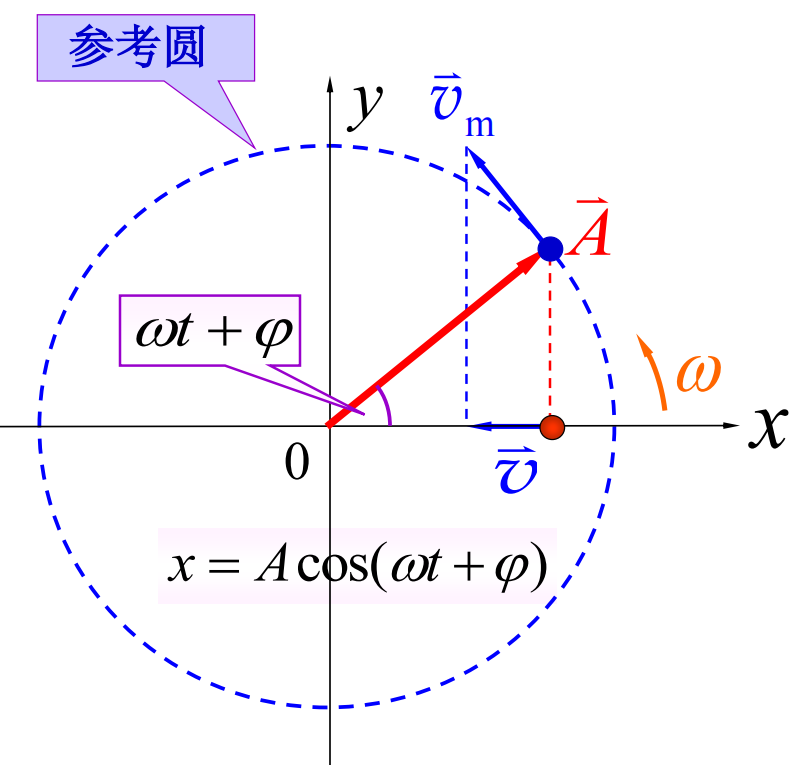
\includegraphics[scale=0.25]{Chapter 06 images/pic3.png}
    \]

    一个动点在参考圆上匀速转动,
    以该动点在参考一个动点在参考圆上匀圆的一根直径上的投影点的运动可代表简谐振动。

\subsubsection{旋转矢量表示法简谐振动}

    \[
        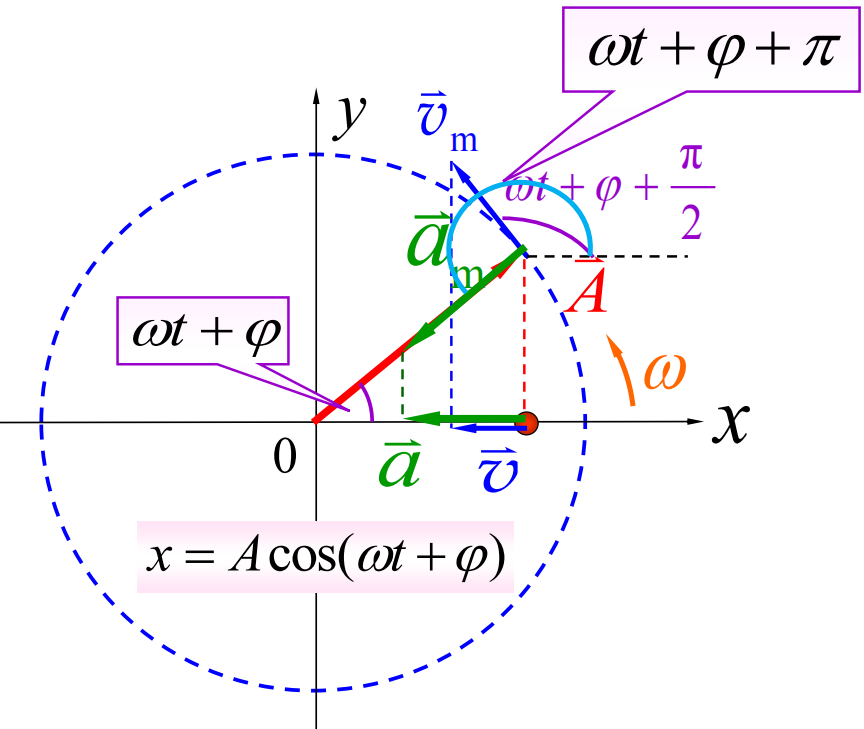
\includegraphics[scale=0.25]{Chapter 06 images/pic4.png}
    \]

    旋转矢量法:矢量\(\overrightarrow{A}\)的端点在\(x\)轴上投影点的运动规律。
    使相位表示更加直观。

    \[
        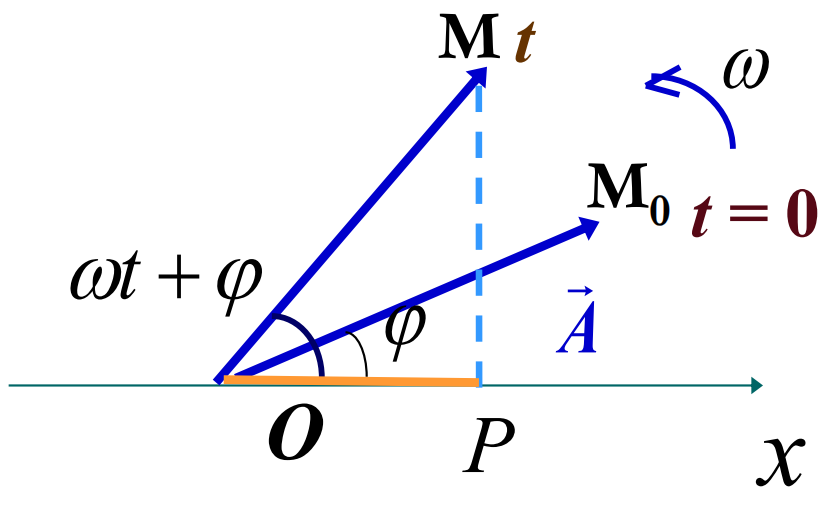
\includegraphics[scale=0.25]{Chapter 06 images/pic5.png}
    \]

    \begin{enumerate}
        \item 在平面图上作一\(Ox\)轴;
        \item 振幅矢量\(\overrightarrow{A}\)从初相位置开始绕\(Ox\)轴上\(O\)点以匀角速度\(\omega\)逆时针旋转,转一圈所用的时间\(T\);
        \item 矢量\(\overrightarrow{A}\)的端点M在\(x\)轴上投影点\(P\)的运动规律:
            \[
                x = A \cos \left(\omega t + \varphi\right)
            \]
    \end{enumerate}

\section{单摆和复摆}

\section{单摆}

    \[
        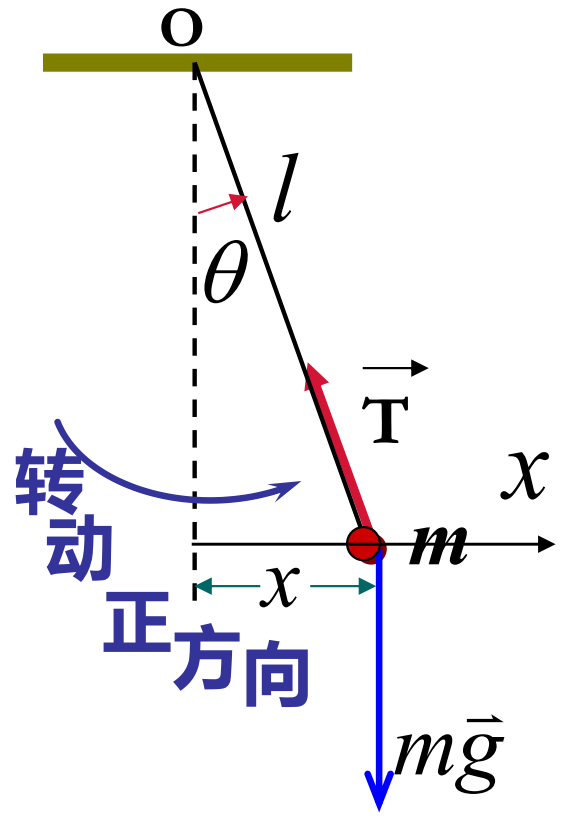
\includegraphics[scale=0.3]{Chapter 06 images/pic6.png}
    \]

    由转动定律,

    \begin{equation}
        M = I \frac{\rmd^2 \theta}{\rmd t^2}
    \end{equation}

    \begin{equation}
        -mg l \sin \theta = m l^2 \frac{\rmd^2 \theta}{\rmd t^2}
    \end{equation}

    当\(\theta < 5\degree\)时,\(\sin \theta \approx \theta\)

    \begin{equation}
        \frac{\rmd^2 \theta}{\rmd t^2} + \frac{g}{l}\theta = 0
    \end{equation}

    即

    \begin{equation}
        \frac{\rmd^2 \theta}{\rmd t^2} + \omega^2 \theta = 0
        \label{6-3-4}
    \end{equation}

    方程\ref{6-3-4}与简谐运动的微分方程式\ref{6-1-2}在数学形式上完全相同。

    在角位移很小的时候,单摆的振动是简谐振动。

    角频率、振动的周期分别为

    \begin{equation}
        \omega = \sqrt{\frac{g}{l}}
    \end{equation}

    \begin{equation}
        T = \frac{2 \uppi}{\omega} = 2 \uppi \sqrt{\frac{l}{g}}
    \end{equation}

    简谐振动表达式为

    \begin{equation}
        \theta = \theta_m \cos \left(\omega t + \varphi\right)
    \end{equation}

\subsection{复摆(刚体的转动)}

    \[
        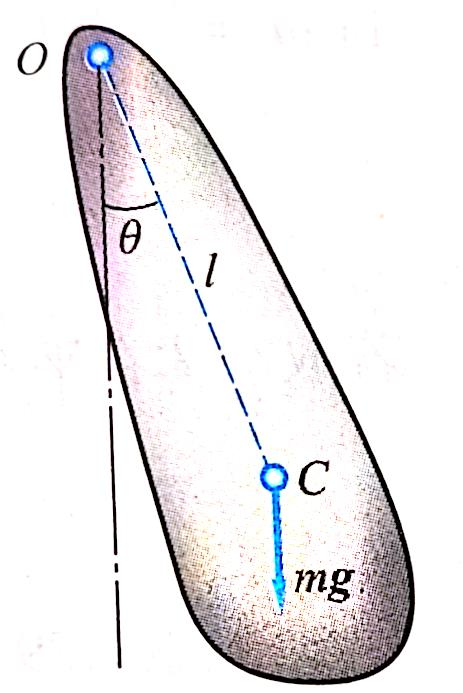
\includegraphics[scale=0.25]{Chapter 06 images/pic7.jpg}
    \]

    一个可绕固定轴\(O\)在竖直平面内摆动的刚体称为复摆 (compound pendulum)。

    \begin{enumerate}
        \item 任意形状;
        \item 小角度;
        \item 无摩擦;
        \item 自由摆动。
    \end{enumerate}

    复摆受重力矩

    \[
        M = -mg l \sin \theta
    \]

    (负号表示重力矩\(M\)的方向与角位移\(\theta\)的方向相反)

    当\(\theta < 5\degree\)时,\(\sin \theta \approx \theta\)

    \[
        M = -mg l \theta
    \]

    由转动定律\(M = I \frac{\rmd^2 \theta}{\rmd t^2}\)

    \begin{equation}
        \frac{\rmd^2 \theta}{\rmd t^2} + \frac{mgl}{I}\theta = 0
    \end{equation}

    在摆角很小时,复摆的运动也是简谐运动,其角频率、振动的周期分别为

    \begin{equation}
        \omega = \sqrt{\frac{mgl}{I}}
    \end{equation}

    \begin{equation}
        T = \frac{2 \uppi}{\omega} = 2 \uppi \sqrt{\frac{I}{mgg}}
    \end{equation}

\subsection{例题}

    长度为\(3a\)的轻质细杆的两端各有质量为\(m\)的小球,该杆可绕水平光滑轴\(O\)
    摆动,若摆角很小,求细杆的振动周期。
    \vspace{1em}

    \textbf{Solution}
    \vspace{1em}

    由转动定律可得

    \[
        -mg \cdot 2a \sin \theta + mg \cdot a \sin \theta = I \frac{\rmd^2 \theta}{\rmd t^2}
    \]

    \[
        I = ma^2 + m\left(2a\right)^2 = 5 ma^2
    \]

    当\(\theta\)很小时时,\(\sin \theta \approx \theta\)

    \[
        \frac{\rmd^2 \theta}{\rmd t^2} + \frac{g}{5a}\theta =0
    \]

    故\(\omega = \dfrac{g}{5a}\),所以

    \[
        T = 2\uppi \sqrt{\frac{5a}{g}}
    \]

\subsection{讨论}

    \begin{enumerate}
        \item 振动系统受弹性回复力之外还受恒力作用时,系统仍作简谐振动。
        \item 质点是绕平衡位置\(O^{\prime}\)作简谐振动的,选平衡位置为坐标原点更方便。
    \end{enumerate}

\end{document}
